\section{Travail réalisé}
\label{p3}
\subsection{Les premiers pas}

Mon stage a commencé par mon immersion dans le projet GDL. Ma première tâche a
consisté à compiler le code source de GDL sur les différentes machines
(\textsc{\small HAKA, ARAMIS\ldots}) avec les différentes options (en
activant ou non certaines bibliothèques externes facultatives). Pour chaque
machine la procédure de compilation a été différente, car les versions de
logiciels/bibliothèques installés ont été différentes ou sur certaines machines
les logiciels/bibliothèques nécessaires pour la compilation n’étaient pas
installés du tout. Les deux cas veulent dire que ça va prendre encore plus du
temps de compiler un projet sur de telles machines. Trouver une version de
logiciel qui va être compatible avec des logiciels/bibliothèques déjà installé
ce n'est pas une tâche triviale d'autant que le projet GDL contient 5 bibliothèques
obligatoires et plus d'une dizaine de bibliothèques optionnelles.

Le build du projet GDL est effectué par \textit{Autotools}, mais dans la version
suivante 0.9.4 \textit{CMake} va remplacer \textit{Autotools}, ce changement est
déjà accompli dans la version CVS du projet. Pour mieux comprendre la raison
pourquoi le projet va abandonner \textit{Autotools} voici le bref description de
ces deux outils:

\begin{description}
\item[Autotools]\hfill \\
Autotools (ou GNU build system) est un ensemble des projets GNU utilisés pour le build de projet sur différents systèmes d'exploitations basés sur Unix; ces outils peuvent être utilisés sur Windows, mais c'est une procédure très restrictive (compilation est possible seulement avec GCC) et prend plus de temps. Il est basé sur shell script, alors il ne nécessite pas l’installation des outils \textit{Autotools} pour faire un build. Ces outils sont très populaires dans le monde Linux. Les outils \textit{Autotools} ont de nombreux inconvénients à cause desquels les développeurs cherchent d'autres solutions. Les problèmes qui repoussent des programmeurs sont:
\begin{itemize}
	\item[$\bullet$] la syntaxe très compliquée, qui rend difficile l’écriture d'un
	script de configuration;
	\item[$\bullet$] large nombre des outils composant avec les syntaxes différents;
	\item[$\bullet$] les messages d'erreurs difficiles à comprendre;
	\item[$\bullet$] création de larges scripts de configuration même pour un
	projet basique;
	\item[$\bullet$] difficilement extensible, difficulté à rajouter des
	fonctionnalités non standard.
\end{itemize}

\item[CMake]\hfill \\
Cross Platform Make ou simplement \textit{CMake} est un moteur de production
créé dans le début des années 2000 pour être compatible avec divers plate-formes
(à peu près tous les systèmes basée sur Unix, Windows: Borland, Visual C++, cygwin\ldots) et divers environnements de développement (KDevelop, XCode, Visual Studio\ldots). Il devient un outils de plus en plus utilisé à cause de ces nombreux avantages:
\begin{itemize}
	\item[$\bullet$] ne dépend que d'un compilateur C++ quelconque;
	\item[$\bullet$] syntaxe très simple à apprendre;
	\item[$\bullet$] il génère un seul Makefile pour touts les plate-formes
	supportées;
	\item[$\bullet$] les messages d'erreurs aident à comprendre le problème;
	\item[$\bullet$] supporte le plate-forme des tests, qui facilite la création des suites des tests;
	\item[$\bullet$] la performance améliorée par rapport aux \textit{Autotools}.
\end{itemize}
Au début de projet GDL l'utilisation de  \textit{CMake} a été impossible à cause de sa licence non compatible avec GPL (GDL utilise la licence GPL), mais la migration sur la licence BSD a aidé à surmonter l'obstacle de non compatibilité. Le point le plus faible de \textit{CMake} représente sa documentation.
\end{description}

Par exemple, si on veut compiler sur \textsc {ARAMIS} la version CVS du projet,
on peut utiliser la suite des commandes suivants (au début on suppose qu'on
est dans la répertoire \textit{{\raise.17ex\hbox{$\scriptstyle\sim$}}/sources/gnudatalanguage/gdl/}):

\lstset{frame=tb,
  language=bash,
  aboveskip=3mm,
  belowskip=3mm,
  showstringspaces=false,
  columns=flexible,
  basicstyle={\ttfamily},
  numbers=none,
  morekeywords={mkdir, cmake, make},
  %numbersep=5pt,
  %numberstyle=\tiny\color{gray},
  rulecolor=\color{black},
  keywordstyle=\color{blue},
  commentstyle=\color{dkgreen},
  stringstyle=\color{mauve},
  breaklines=true,
  breakatwhitespace=true
  tabsize=3,
}

\begin{lstlisting}
mkdir compil build
cd compil
cmake .. -DHDF=OFF -DPSLIB=OFF -DPLPLOTDIR=~/sources/plplot-5.9.6/build/ 
-DCMAKE_INSTALL_PREFIX=~/sources/gnudatalanguage/gdl/build/ 
make -j 8
make check
\end{lstlisting}


\subsection{Fonction d'inversion de matrice}

\subsubsection{Contexte}

Ma première mission d’écriture de code a été le développement de la fonction
d'inversion de matrice. En fait la fonction d’inversion de matrice
(INVERT) était déjà présente dans le projet GDL, mais elle a été écrite en
utilisant la librairie GSL (GSL représente des outils de calculs numériques en
mathématiques appliquées, elle fait partie du projet GNU et est distribuée selon
les termes de la licence GNU GPL). Depuis début 2013, l’équipe GDL mène des essaies très fructueux avec la librairie Eigen. INVERT est un code important, il fallait voir si un gain de temps notable existe avec Eigen par rapport à la GSL. Alors j'ai dû réécrire INVERT en utilisant la librairie Eigen (librairie de C++ contenant des templates qui implémentent l’algèbre linaire et des opérations sur les matrices, sous la licence libre MPL2, qui représente l'hybride de BSD et GPL).

\subsubsection{Réalisation}
La philosophie de GDL est directement inspirée du monde libre, ainsi, si un code
existe déjà et qu’il est possible de l’intégrer dans le projet grâce à sa
licence, il est inutile de perdre du temps à le réécrire. On peut aussi choisir
entre plusieurs librairies externes en fonction de critères: simplicité,
taille, performance, évolution. C'est pourquoi, plutôt que de coder l’algorithme
d'inversion de matrice j'ai préféré utiliser les routines existantes et largement testées.

Dans la fonction d'inversion, la matrice est donnée sous les types du langage
C/C++. Pour mieux traiter les données Eigen a ses propres types de données et
pour convertir les donnée existant de type non-Eigen à un type interne d'Eigen
on a le mapping. La classe Map de bibliothèque Eigen contient des routines de
mapping. Ces routines sont trés simples à utiliser et elles sont très performantes.

Exemple de mapping:

\lstset{frame=tb,
  language=C++,
  aboveskip=3mm,ils
  belowskip=3mm,
  showstringspaces=false,
  columns=flexible,
  basicstyle={\ttfamily},
  numbers=none,
  morekeywords={Map,MatrixXf},
  %numbersep=5pt,
  %numberstyle=\tiny\color{gray},
  rulecolor=\color{black},
  keywordstyle=\color{blue},
  commentstyle=\color{dkgreen},
  stringstyle=\color{mauve},
  breaklines=true,
  breakatwhitespace=true
  tabsize=3,
}

\begin{lstlisting}
float array[rows*cols];
Map<MatrixXf> m(array,rows,cols);
\end{lstlisting}


\subsubsection{Tests}

Avant de publier dans le CVS la nouvelle fonction d'inversion d'une matrice il faut la bien tester. Les tests sont nombreux et divers: 

\begin{itemize}
	\item[$\bullet$] tests de justesse,
	\item[$\bullet$] tests de types,
	\item[$\bullet$] tests de correspondance avec la syntaxe IDL,
	\item[$\bullet$] tests de performance.
\end{itemize}

Ces tests sont nécessaires pour assurer la qualité de projet et d’éviter les problèmes dans le futur. Les résultats des tests de performance seront discutées dans la section suivante.

\subsection{Nombre de threads}
\label{num_thread}

\subsubsection{Contexte}
Quand la fonction d'inversion de matrice utilisant la librairie Eigen (INVERT\_EIGEN) a été prête, ses benchmarcks sur une machine chargée ont montré un résultat complètement différent de celui de la machine non chargée. Par rapport à IDL la même fonction d'inversion de matrice sur une machine non chargée a été plus rapide pour tous les types, mais sur la machine chargée (même s'il y a eu un seul cœur occupé et 15 disponibles) pour certaines types la performance a baissé de 10 fois ou même plus. D’après l'analyse de la documentation de la librairie Eigen et la consultation (par courriel électronique) avec les autres membres de la communauté (Marc Schellens, Gilles Duvert\ldots) on a trouvé que le problème est causé par le nombre de threads défini statiquement et indépendant de la charge de machine pour OpenMP (Eigen utilise OpenMP pour bénéficier des multi-cœurs).

Cette occasion a produit un devoir inattendu: j'ai dû écrire une fonction qui va définir le nombre de threads dynamiquement avant chaque exécution du GDL et cette fonction va prendre en considération la charge de la machine sur laquelle elle est exécutée.

\subsubsection{Réalisation}
Sous les systèmes d'exploitations basées sur Unix on calcule le nombre de threads optimal (\textit{suggested\_num\_threads}) par la formule suivante:

\begin{equation}
	\large
	suggested\_num\_threads=nbofproc-avload
   	\label{form:num_threads_u}
\end{equation}

Le nombre de processeurs sur la machine (\textit{nbofproc}) est connu pour OpenMP et c'est un simple appel à sa fonction interne. Alors, il nous reste de trouver la charge moyenne de la machine (\textit{avload}). La charge moyenne de la machine est définie comme un nombre réel de type X.XX (par exemple: \textit{avload}=2.64 sur une machine avec 8 processeurs virtuels, où 2 signifie, que deux processeurs sont entièrement occupés et .64 signifie, que le troisième est chargé partiellement; les cinq processeurs sont libres), de dernière(s) 1, 5 ou 15 minutes. Dans notre cas on a décidé d'utiliser le moyen de 5 derniers minutes, car une minute c'est un intervalle très court pour faire une conclusion sur la charge de la machine et 15 minutes c'est trop long (on veut pas prendre en compte la charge de la machine par un logiciel qui a déjà terminé son fonctionnement). Puisque le nombre de processeurs est un nombre entier et la charge moyenne est un nombre réel, la valeur de la charge moyenne est arrondi au plus proche.

Sous le système d'exploitation Windows le nombre de threads optimal est calculé par la formule un peu différente:
\begin{equation}
	%\Large
	suggested\_num\_threads = nbofproc - avload * nbofproc/100
  	\label{form:num_threads_w}
\end{equation}

La différence vient du format de présentation de charge de la machine, qui est représenté sous Windows comme un pourcentage d'occupation de tous les processeurs virtuels (par exemple: \textit{avload}=50 sur une machine avec 8 processeurs virtuels signifie que 4 processeurs sont occupés et les 4 restants sont libres).

Le code source de la fonction \textit{set\_num\_threads} est disponible dans l'Annexe \ref{code_num_threads} sur page \pageref{code_num_threads}.


\subsubsection{Étude des performances}
%\vspace{2\baselineskip}\vspace{-\parskip}

L’aspect très important dans la concurrence entre GDL et IDL c'est la performance, afin qu'ils sont utilisés pour les calculs scientifiques. Signifiant, que les données à traiter sont assez larges (par exemple: les matrices avec des dimensions supérieures à 200). La performance de la majorité des fonctions de GDL est très proche ou même meilleure que la performance d'IDL, mais pour attirer plus d'utilisateurs il faut avoir un meilleur indice de performance que IDL pour tous les fonctions sur tous les systèmes d'exploitations.

Pour trouver les indices de performance des différents fonctions d'inversion de matrice une suite de tests a été écrite, ces tests se composent de calcul du temps d'inversion des matrices aux très larges dimensions (255, 256, 300, 500). Les tests ont été faits sur \textsc{ARAMIS}, qui pour le moment de tests a eu 2 cœurs occupés en permanence par des autres processus. Cette condition a été idéale pour tester la performance de cette nouvelle caractéristique qui a été introduite par la fonction de définition de nombre de threads.

D’après les tests, la fonction d'inversion de matrice utilisant la bibliothèque Eigen donne une meilleur performance que celle utilisant la bibliothèque GSL. Mais sur une machine chargée les deux fonctions deviennent incomparable avec la fonction de IDL, qui est largement plus rapide. Alors, après la fonction \textit{set\_num\_threads} la performance de la fonction d'inversion de matrice avec GSL (qui est utilisé dans la plupart de fonctions codés sous C++ pour les calcules scientifiques) est proche de la fonction présent dans IDL et parfois est meilleur.

Une fois les problèmes du nombre des threads optimale sont réglés, la fonction d'inversion de matrice avec Eigen a les meilleurs résultats pour touts les types (la Table \ref{test_perf} montre les temps de calcul pour les multiples fonctions). En plus d'une bonne performance, Eigen est simple à utiliser et il se charge de la gestion de la mémoire, qui dispense l'utilisateur de gérer les éventuelles fuites mémoire. C'est pourquoi Eigen a été choisi comme une bibliothèque pour les calculs matriciels pour les nouvelles fonctionnalités, qui vont faire partie de GDL version 0.9.4.\\

En conséquence, la définition dynamique du nombre de threads a permis d'obtenir un meilleur indice de performance pour l'inversion de matrice aussi bien que pour tous les fonctions utilisant la parallélisation avec OpenMP dès que les machines sont un peu chargées.

\renewcommand{\arraystretch}{1.3}
\begin{table}
\begin{center}
\renewcommand{\thefootnote}{\alph{footnote}}
    %\begin{adjustwidth}{-0.7in}{-1in}
    \begin{tabular}{  c | c | c | c | c | c |}
    \cline{2-6}
      & \multicolumn{2}{ | c | }{GDL INVERT\footnotemark[1]} & \multicolumn{1}{ | c | }{\multirow{2}{*}{IDL}} & \multicolumn{2}{ | c | }{GDL INVERT\footnotemark[2]} \\
    \cline{1-3}
    \cline{5-6}
    \multicolumn{1}{ |c| }{Type} 	& GSL 	& EIGEN &  		& GSL 	& EIGEN \\ \hline
    \multicolumn{1}{ |c| }{BYTE}	& 7.383 & 6.249 & 0.543 & 0.663 & 0.397	\\ \hline
    \multicolumn{1}{ |c| }{INT}		& 5.242 & 6.125	& 0.530 & 0.657 & 0.374	\\ \hline
    \multicolumn{1}{ |c| }{LONG} 	& 5.108	& 5.605	& 0.537 & 0.656 & 0.365	\\ \hline
    \multicolumn{1}{ |c| }{FLOAT} 	& 7.768	& 5.283	& 0.533 & 0.630 & 0.339	\\ \hline
    \multicolumn{1}{ |c| }{DOUBLE} 	& 5.645	& 6.580	& 1.161 & 0.690 & 0.466	\\ \hline
    \multicolumn{1}{ |c| }{COMPLEX} & 10.218& 9.467 & 3.991 & 2.004 & 1.651	\\ \hline
    \multicolumn{1}{ |c| }{DCOMPLEX} & 13.543& 2.675& 4.365 & 2.160 & 2.089	\\ \hline
    \multicolumn{1}{ |c| }{UINT} 	& 9.204	& 7.416 & 0.520 & 0.671 & 0.399	\\ \hline
    \multicolumn{1}{ |c| }{ULONG} 	& 5.546	& 5.238 & 0.522 & 0.666 & 0.397	\\ \hline
    \end{tabular}
        %\end{adjustwidth}
\end{center}
        
        \caption*{de
        \footnotetext[1]{sans \textit{set\_num\_threads} sur une machine chargé}
        \footnotetext[2]{avec \textit{set\_num\_threads} ou sans \textit{set\_num\_threads}, mais sur une machine non chargée}
        }
        \caption{Résultats des tests de performance sur la fonction INVERT, utilisant la GSL ou Eigen}
        \label{test_perf}
\end{table}



\newpage
\subsection{Factorisation de Cholesky}

\vspace{1\baselineskip}\vspace{-\parskip}

La tâche suivante a été de coder sous C++ la factorisation (décomposition) de
Cholesky d'une matrice. Dans IDL on a quatre procédures/fonctions concernant la
factorisation de Cholesky (CHOLDC, CHOLSOL, LA\_CHOLDC, LA\_CHOLSOL). Tous ces
procédures/fonctions étaient absentes dans GDL et des utilisateurs souhaitent en
bénéficier. Certaines codes en syntaxe IDL/GDL (PlanckSkyModel, iCosmo)
utilisent CHOLDC et ne pouvaient être totalement audités. Ma mission a été de
les rajouter en utilisant la bibliothèque Eigen.

Cette factorisation est utilisée pour la résolution des systèmes d'équations linéaires, simulations avec méthode de Monte-Carlo, filtre de Kalman, l'inversion d'une matrice hermitienne.\\

\subsubsection{Description de factorisation de Cholesky}

\vspace{1\baselineskip}\vspace{-\parskip}

La factorisation de Cholesky, nommée d'après André-Louis Cholesky, consiste, pour une matrice symétrique définie positive \textbf{A}, à déterminer une matrice triangulaire inférieure \textbf{L} telle que :
\begin{equation}
	%\Large
	A=LL^T
  	\label{form:cholesky}
\end{equation}

Ou \textbf{L\textsuperscript{T}} est la transposée de la matrice triangulaire inférieure \textbf{L}. On peut imposer que les éléments diagonaux de la matrice \textbf{L} soient tous positifs, et la factorisation correspondante est alors unique.\\

\begin{figure}[!ht]
    \centerline{
    	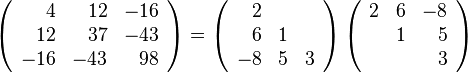
\includegraphics[width=0.8\textwidth]{./images/ex_chol.png}
    	}
    \caption{Exemple de factorisation de Cholesky}
	%\centerline{Source - http://upload.wikimedia.org/math/9/7/3/9733349e9de16e972daca756204d97db.png}
    \label{ex_chol}
\end{figure}

Pour la résolution d'un système d'équations linéaires, la factorisation de Cholesky est approximativement deux fois plus efficace que la décomposition LU. Alors c'est très important d'avoir dans GDL les routines concernant la factorisation de Cholesky.

\subsubsection{La réalisation de CHOLDC, CHOLSOL}

Le première ensemble de factorisation de Cholesky que j'ai codé a été la
procédure \textbf{CHOLDC}. Cette procédure est utilisée pour trouver une matrice
triangulaire inférieure d'une matrice symétrique définie positive donnée. Coder cette procédure a été une tâche sans peine, car j'ai déjà eu l’expérience de codage avec la librairie Eigen, que j'ai obtenu pendent ma mission précédent (la fonction d'inversion de matrice). En plus Eigen contient tous les algorithmes de suite de Cholesky, alors j'ai dû à faire la répartition des appels des algorithmes pour les types appropriés du coté de GDL.

Ensuite j'ai implémenté la fonction \textbf{CHOLSOL}. Cette fonction calcule la
solution pour un système d'équations linéaires \textbf{Ax=B}. Cette fonction
prend comme premier argument la matrice calculée par \textbf{CHOLDC}, mais GDL en différence d'IDL utilise la matrice triangulaire supérieure qui contient les valeurs initiales. La différence est à cause de librairie Eigen, qui ne support pas la résolution d'un système d'équations linéaires d’après les valeurs intermédiaires (la matrice décomposée). \\

\begin{figure}[!ht]
\centering
	\begin{subfigure}[b]{0.6\textwidth}
    	\centering
    		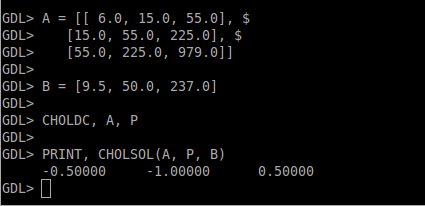
\includegraphics[width=\textwidth]{./images/ex_chols.png}
    		 \caption{GDL}
    		 \label{ex_chols_gdl}
    \end{subfigure}
    ~
    \begin{subfigure}[b]{0.6\textwidth}
    	\centering
    		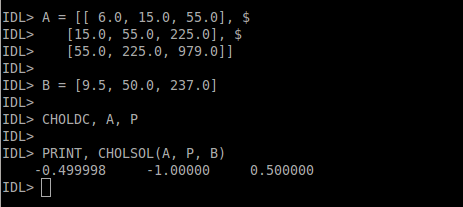
\includegraphics[width=\textwidth]{./images/ex_chols_idl.png}
    		\caption{IDL}
    		\label{ex_chols_idl}
    \end{subfigure}
    
    \caption{Exemple de résolution d'un système d'équations linéaires dans les interpréteurs GDL et IDL}
	%\centerline{Source - capture d'ecran}
    \label{ex_chols}
\end{figure}

La Figure \ref{ex_chols}\ montre un exemple de résolution d'un système
d'équations linéaires \textbf{Ax=B}\ dans différents interpréteurs en utilisant
la procédure \textbf{CHOLDC} et ensuite la fonction \textbf{CHOLSOL}. Pour
résoudre un système d'équations linéaires dans IDL on est obligé d’exécuter les
deux procédures, mais dans GDL on peut le résolve sans utilisation de
\textbf{CHOLDC}. Puisque dans la fonctions \textbf{CHOLSOL} on fait la
décomposition (c'est obligatoire en raison d'utilisation de la bibliothèque Eigen).
Pour assurer la compatibilité on peut résoudre \textbf{Ax=B}\ à la manière d'IDL
(suite de deux commandes).

La besoin de calculer deux fois la même factorisation baisse la performance de
GDL  dans résolution d'un système d'équations linéaires, mais GDL a un autre avantage par rapport à IDL: c'est une solution plus exacte. Dans un exemple qui est représenté sur la Figure \ref{ex_chols}\ la solution exacte est un vecteur avec les valeurs: \{ -0.500000, -1.00000, 0.500000 \} - ce que retourne GDL, mais le vecteur calculé par IDL est un peu différent, la première valeur contient un erreur de -0.000002.

\subsubsection{La réalisation de LA\_CHOLDC, LA\_CHOLSOL}

La procédure \textbf{LA\_CHOLDC} est la procédure \textbf{CHOLDC} généralisée
pour trouver la décomposition d'une matrice à coefficients complexes (matrice hermitienne). Pour la factorisation d'une matrice à coefficients réels, en plus de la formule \eqref{form:cholesky} (page \pageref{form:cholesky}) qui est utilisée par la procédure \textbf{CHOLDC}, \textbf{LA\_CHOLDC} peut utiliser la formule \eqref{form:cholesky-sup}, ou \textbf{U} est une matrice triangulaire supérieur et \textbf{U\textsuperscript{T}} est sa transposée:
\begin{equation}
	%\Large
	A=U^TU
  	\label{form:cholesky-sup}
\end{equation}

Pour une matrice hermitienne la procédure \textbf{LA\_CHOLDC} peut utiliser l'une des formules suivantes:

 \begin{equation}
	%\Large
	A=U^HU
  	\label{form:cholesky-com-sup}
\end{equation}

 \begin{equation}
	%\Large
	A=LL^H
  	\label{form:cholesky-com}
\end{equation}

\textbf{H} signifie une matrice adjointe (aussi appelée matrice transconjuguée).

La réalisation de \textbf{LA\_CHOLDC} a été similaire à la réalisation de
\textbf{CHOLDC}, car la bibliothèque Eigen gère les types complexes aussi bien que les autres types.

Le code complet des routines Cholesky est disponible dans le CVS du projet \url{http://smarturl.it/Cholesky}

\subsection{Convolution}
\subsubsection{Contexte}
La procédure \textbf{CONVOL} convole un tableau (1D, 2D, 3D\ldots) avec un noyau et retourne un tableau modifié. La convolution est largement utilisée dans divers domaines des sciences pour traitement d'image, traitement de signal, différenciation et beaucoup d'autres opérations. Le traitement d'images fait un grand partie d'astronomie, comme les image obtenu par les satellites parfois ont des défauts, on a besoin d'une procédure de correction. Alors c'est très important d'avoir la procédure de convolution dans GDL.


\begin{figure}[!ht]
    \centerline{
    	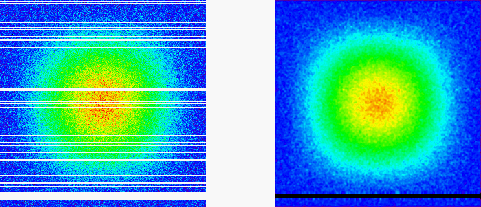
\includegraphics[width=0.8\textwidth]{./images/convol_example2.png}
    	}
    \caption{Exemple d'utilisation de convolution en traitement d'image en IDL. Cette fonctionnalité n'est pas encore disponible dans GDL}
	%\centerline{Source - http://www.exelisvis.com/docs/html/images/convol_example2.gif}
    \label{ex_convol_img}
\end{figure}

La Figure \ref{ex_convol_img} est un exemple de lissage d'image bruitée avec les données manquantes. Après la procédure de convolution la majorité des  données manquant est restauré et le bruit est réduit. On peut appliquer les différents effets sur cette image, l'effet est défini par le noyau (aussi appelé filtre) avec le-quelle image est convolé.

\begin{figure}[!ht]
\centering
	\begin{subfigure}[b]{0.3\textwidth}
    	\centering
    		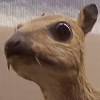
\includegraphics[width=\textwidth]{./images/ex_edge_or.png}
    		 \caption{Originale}
    		 \label{ex_edge_or}
    \end{subfigure}
    ~~
    \begin{subfigure}[b]{0.3\textwidth}
       	\centering
       		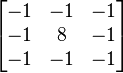
\includegraphics[width=\textwidth]{./images/filtre.png}
       		 \caption{Filtre}
       		 \label{ex_edge_fi}
    \end{subfigure}
    ~~
    \begin{subfigure}[b]{0.3\textwidth}
    	\centering
    		
\includegraphics[width=\textwidth]{./images/ex_edge_ch.png}
    		\caption{Après la convolution}
    		\label{ex_edge_ch}
    \end{subfigure}
        \caption{Exemple d'utilisation de convolution pour détecter les contours}
    \label{ex_edge}
\end{figure}

\subsubsection{Réalisation}
La fonction de convolution est présente dans GDL depuis 2004, mais elle est resté inchangée malgré les changements dans cette fonction dans IDL (nouveaux mot-clés ajoutés). D'ajouter la prise en compte effective de certaines nouveaux mot-clés dans \textbf{CONVOL} de GDL m'a été confié. J'ai commencé la mise à jour de cette fonction par regroupement de plusieurs fonctions concernant la convolution dans un même fichier. Cette stratégie est efficace pour le gain du temps et compréhension de vieux code afin qu'on ne cherche pas les parties du code.

Le code complet de fonction \textbf{CONVOL} avec tous les mot-clés déjà ajoutés est très large et la compréhension du code a pris beaucoup de temps. L’étude de code m'a pris environs une semaine. En plus des difficultés pour comprendre le code, comme il n'est pas en maintenance depuis longtemps la partie de code a perdu son efficacité. Donc, trouver les parties faibles du code et les corriger a fait la partie de cette mission.

Pendant la réalisation de mis à jour de la fonction de convolution la tâche le plus difficile a été d'assurer son fonctionnement pour tous les types. La grande partie du code est généralisé pour tous les types (en utilisant les Templates). Mais, comme les différents types ont différents caractéristiques on a eu besoin de réécrire la partie de la logique plusieurs fois en fonctionnement du type utilisé et pendant la compilation inclure le code approprié à ce type. Par exemple le fait que les nombres complexes n'ont pas d'ordre a causé des problèmes quand on a eu besoin de les comparer.

Le code de la fonction de convolution est dans l'Annexe \ref{code_convol}, page \pageref{code_convol}. Ce code ne représente pas le code complet de \textbf{CONVOL} de GDL, le code complet est disponible dans le CVS du projet \url{http://smarturl.it/Convol}

\subsubsection{Tests}

Des tests pour la convolution étaient absent dans la suite de tests du projet. Alors j'ai écrit des tests en syntaxe IDL/GDL pour assurer que tous les types sont bien gérés. Après l'application de ce test aux différents environnements, on a trouvé que les type \textbf{ULONG, ULONG64} ont des problèmes avec GCC version jusqu'à 4.4 et le projet ne compile pas. Pour l'instant ces deux types sont interdits dans \textbf{CONVOL}.

\subsection{Correction de bugs}

Pendant mon stage dans l’interval entre les grandes missions j'ai eu des "petit" tâches. Ces tâches comprennent la correction de divers bugs dans GDL. L'un de ces bug a été un problème typique du langage C++ - fuite mémoire (appel de \textbf{delete[]} pour libérer la mémoire alloué par \textbf{new}). Un autre crash de GDL était causé par la copie de bloc de mémoire de \textbf{long} à \textbf{double}. Ces deux types ont les longueurs différentes pour les différentes architectures (32/64 bits). Sur une architecture de 32 bits les deux ont la longueur maximale de 32 bits, mais sur l'architecture de 64 bits ils ont les longueurs différentes (\textbf{long} - 32 bits, \textbf{double} - 64 bits). Ces fuites mémoire ont été trouvées grâce au logiciel Valgrind.

J'ai aussi corrigé un bug dans le code de build en syntaxe CMake. Le projet GDL utilise les bibliothèques ImageMagick ou GraphicsMagic, la deuxième est plus prioritaire. CMake n'arrive pas à trouver si ImageMagick est installé dans un répertoire différent de celui par défaut. En analysant le code j'ai trouvé que le problème venait des versions récentes de ImageMagick ou le nom du répertoire a été changé. C'est un problème classique, quand les deux logiciels ne sont pas en accord.

Un dernier bug significatif concernait un traitement d'une chaîne de caractères dans GDL. Le traitement marchait jusqu'au premier espace blanc, j'ai ajouté une boucle pour passer toute la chaîne de caractères. Cette modification a amélioré les appels des commandes d'interpréteur de commandes système (par exemple: \textbf{cd, cp, mkdir \ldots}).









